\section{Fibonacci Heaps}
Okaaaaaay! This is awesome! Kick some serious ass!
%
\subsubsection{Mergeable Heaps}
A mergeable heap is any data structure that supports the following five operations in which each has a key:

\begin{footnotesize}
\begin{itemize}
	\item MAKE-HEAP() creates and returns a new heap containing no elements
	\item INSERT($H, x$) inserts an element $x$, whose $key$ has already been filled in, into heap $H$
	\item MINIMUM($H$) returns a pointer to the element in heap $H$ whose key is minimum
	\item EXTRACT-MIN($H$) deletes the element from heap $H$ whose key is minimum, returning a pointer to the element
	\item UNION($H_1, H_2$) creates and returns a new heap that contains all the elements of heaps $H_1$ and $H_2$. Heaps $H_1$ and $H_2$ are ``destroyed'' by this operation
\end{itemize}
\end{footnotesize}

Besides the mergeable-heap operations above, Fibonacci heaps also support the following two operations:

\begin{footnotesize}
\begin{itemize}
	\item DECREASE-KEY($H, x, k$) assigns to element $x$ within heap $H$ the new key value $k$, which we assume to be no greater than its current value
	\item DELETE($H, x$) deletes element $x$ from heap $H$
\end{itemize}
\end{footnotesize}

\begin{footnotesize}
\begin{table}[H]
\center
\begin{tabular}{l c c}
 & Binary heap & Fibonacci heap \\
 Procedure & (worst case) & (amortised)\\
\hline
MAKE-HEAP 		& $\Phi(1)$ 		& $\Phi(1)$\\
INSERT 			& $\Phi(\lg(n))$ 	& $\Phi(1)$\\
MINIMUM			& $\Phi(1)$		& $\Phi(1)$\\
EXTRACT-MIN		& $\Phi(\lg(n))$	& $O(\lg(n))$\\
UNION			& $\Phi(n)$		& $\Phi(1)$\\
DECREASE-KEY	& $\Phi(\lg(n))$	& $\Phi(1)$\\
DELETE			& $\Phi(\lg(n))$	& $O(\lg(n))$
\end{tabular}
\caption{Running times for operations on two implementations of mergeable heaps. The number of items in the heap(s) at the time of an operation is denoted by $n$}
\end{table}
\end{footnotesize}
%
\subsubsection{Fibonacci heaps in theory and practice}
Fibonacci heaps are theoretically desirable when the number of EXTRACT-MIN and DELETE operations is small relative to the number of other operations performed. This can be the case for some algorithms in graph problems, that call DECREASE-KEY once per edge. Fast algorithms for computing minimum spanning trees and finding single-source shortest paths make essential use of Fibonacci heaps.\\

From a practical point of view, however, the constant factors and complexity of Fibonacci heaps make them less desirable than ordinary binary (or $k$-ary) heaps for most applications. As such, Fibonacci heaps are pre-dominantly of theoretical interest.
%
\subsection{Structure of Fibonacci Heaps}
A Fibonacci Heap is a collection of rooted trees that are min-heap ordered. That is, each tree obeys the min-heap property: the key of a node is greater than or equal to the key of its parent. Each node contains a pointer to its parent and a pointer to any one of its children. The children are linked together in a circular, doubly linked list. In a circular, doubly linked list we can insert a node into any location or remove a node from anywhere in the list in $O(1)$ time. We can also concatenate two such lists in $O(1)$ time.
\begin{figure} [H]
    \begin{center}
        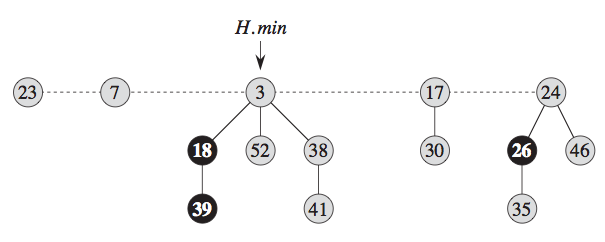
\includegraphics[width=\textwidth]{Images/Hmin.png}
        \caption{Fibonacci heap consisting of five min-heap-ordered trees and 14 nodes}
        \label{fig:H.min}
    \end{center}
\end{figure}

We store the number of children in the cild list of node $x$ in $x.degree$. The boolean-valued attribute $x.mark$ indicates whether node $x$ has lost a child since the last time $x$ was made the child of another node. Newly created nodes are unmarked, and a node becomes unmarked whenever it is made the child of another node. Root nodes are unmarked.\\

We access a Fibonacci heap $H$ by a pointer $H.min$ to the root of a tree containing the minimum key; we call this node the \textit{minimum node} of the Fibonacci heap.\\

The roots of all the trees in a Fibonacci heap are linked together using their left and right pointers into a circular, doubly linked list called the \textit{root list} of the Fibonacci heap. Finally, $H.n$ refers to the number of nodes currently in the heap.
%
\subsubsection{Potential Function}
In the following, the potential function of fibonacci heap is defined by
\begin{align}
	\Phi(H) = t(H) + 2m(H)
\end{align}
where $t(H)$ is the number of trees in the root list and $m(H)$ is the number of marked nodes. The potential function captures the state of a system at a given point, and we can then calculate an amortised\footnote{Amortiseret = Udover n operationer, så er det gennemsnittet} time as the actual time plus a constant times the change in state ‘energy’. This provides a valid upper bound on running time.

\subsubsection{Maximum Degree}
Meeh, nothing important, I think... 

\subsection{Mergeable-heap Operations}
The mergeable-heap operations on Fibonacci heaps delay work as long as possible. We shall see that, no matter what the root list looks like before a EXTRACT-MIN operation, afterward each node in the root list has a degree that is unique within the root list, which leads to a root list of size at most $D(n) + 1$. 
%
\subsubsection{Creating a New Fibonacci Heap}
To make an empty Fibonacci heap, the MAKE-FIB-HEAP procedure allocates and returns the Fibonacci heap object $H$, where $H.n = 0$ and $H.min = NIL$; there are no trees in $H$. Because $t(H) = 0$ and $m(H) = 0$, the potential of the empty Fibonacci heap is $\Phi(H) = 0$. The amortised cost of MAKE-FIB-HEAP is thus equal to its $O(1)$ actual cost.
%
\subsubsection{Inserting a Node}
\begin{figure} [H]
    \begin{center}
        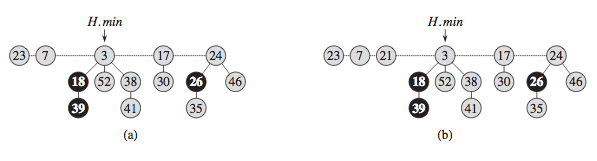
\includegraphics[width=\textwidth]{Images/InsertFib.png}
        \caption{\footnotesize{Inserting a node into a Fibonacci heap. \textbf{(a)} A Fibonacci heap $H$. \textbf{(b)} Fibonacci heap $H$ after inserting the node with key 21. The node becomes its own min-heap-ordered tree and is then added to the root list, becoming the left sibling of the root.}}
    \end{center}
\end{figure}

To determine the amortised cost of FIB-HEAP-INSERT, let $H$ be the input Fibonacci heap and $H'$ be the resulting Fibonacci heap. Then $t(H') = t(H) + 1$ and $m(H') = m(H)$, and the increase in potential is $((t(H) + 1) + 2m(H)) - (t(H) + 2m(H)) = 1$. \\

Since the actual cost is $O(1)$, the amortised cost is $O(1) + 1 = O(1)$.
%
\subsubsection{Finding the Minimum Node}
The minimum node of a Fibonacci heap $H$ is given by the pointer $H.min$, so we can find the minimum node in $O(1)$ actual time. Because the potential of $H$ does not change, the amortised cost of this operation is equal to its $O(1)$ actual cost. 
%
\subsubsection{Uniting Two Fibonacci Heaps}
We simply concatenate the root lists of $H_1$ and $H_2$ and then determines the new minimum node. Afterward, the objects representing $H_1$ and $H_2$ will never be used again. \\

The change in potential is\\ $\Phi(H) - (\Phi(H_1) + \Phi(H_2)) = (t(H) + 2m(H)) - ((t(H_1) + 2m(H_1)) + (t(H_2) + 2m(H_2))) = 0$\\ because $t(H) = t(H_1) + t(H_2)$ and $m(H) = m(H_1) + m(H_2)$. The amortised cost of FIB-HEAP-UNION is therefore equal to its $O(1)$ actual cost. 
%
\subsubsection{Extracting the Minimum Node}
The process of extracting the minimum node is the most complicated of the operations presented in this section. It is also where the delayed work of consolidating trees in the root list finally occurs. \\

FIB-HEAP-EXTRACT-MIN works by first making a root out of each of the minimum node’s children and removing the minimum node from the root list. It then consolidates the root list by linking roots of equal degree until at most one root remains of each degree.\\

Consolidating the root list consists of repeatedly executing the following steps until every root in the root list has a distinct degree value:
\begin{enumerate}
	\item Find two roots $x$ and $y$ in the root list with the same degree. Without loss of generality, let $x.key \leq y.key$
	\item \textbf{\textit{Link}} $y$ to $x$: remove $y$ from the root list, and make $y$ a child of $x$ by calling the FIB-HEAP-LINK procedure. This procedure increments the attribute $x.degree$ and clears the mark on $y$. 
\end{enumerate}

So what we do is, removing $H.min$ and add its children to the root list. Then we start the consolidation with array $A$, starting at the new $H.min$ going to right. When we have to nodes with same degree (height) in a row, we merge them. In the end we have a bunch of nodes at the root list with different degrees, and we mark the new $H.min$. \\

There are several things we must estimate the cost of: extracting the minimum node, the main for-loop through the root list and within that the while-loop that links together trees.\\

The amortised cost of extracting the minimum node of an n-node Fibonacci heap is $O(D(n))$. Let $H$ denote the Fibonacci heap prior to the ExtractMin operation. The actual cost of extracting the minimum node contributes $O(D(n))$ work from processing at most $D(n)$ children of the minimum node.\\

Upon calling consolidate, the size of the root list is at most $D(n) + t(H) - 1$: the original $t(H)$ root-list nodes, minus the extracted root node, plus the children of the extracted node, at most $D(n)$. Every iteration of the inner while-loop, we know that one root is linked to another, and so the total number of iterations of the while loop over all iterations of the for loop is at most the number of roots in the root list. Hence, the total amount of work performed in the for loop is at most proportional to $D(n)+ t(H)$. The total actual work in extracting the minimum node is therefore $O(D(n) + t(H))$. The potential before extracting the minimum node is $t(H) + 2m(H)$. The potential afterwards is at most $(D(n) + 1) + 2m(H)$, since at most $D(n) + 1$ roots remain and no nodes get marked during this operation. The amortised cost is thus at most:
\begin{align*}
	&O(D(n) + t(H)) + ((D(n) + 1) + 2m(H)) - (t(H) + 2m(H))\\
	&= O(D(n)) + O(t(H)) - O(t(H))\\
	&= O(D(n))
\end{align*}
if we scale up the units of the potential to dominate the constant hidden in $t(H)$. We will see later that $D(n) = O(\lg n)$, giving an amortised running time of $O(\lg n)$ for extracting the minimum node.
%
\subsection{Decreasing a Key and Deleting a Node}
\subsubsection{Decreasing a Key}
To decrease a key a few things happens. We start with an initial Fibonacci heap. It is important to notice the marked nodes. A node is now decreased and it is moved to the root list, and its parent is marked. IF the parent was marked already, the marked parent is cut from its own parent and moved to the root list unmarked. When we reach an unmarked node or a root key, the algorithm stops, and we update $H.min$ if necessary. \\

The FIB-HEAP-DECREASE-KEY procedure takes $O(1)$ time plus the time to perform the cascading cuts. Suppose that a given invocation of FIB-HEAP-DECREASE-KEY results in $c$ calls of CASCADING-CUT - each of these calls takes $O(1)$ time exclusive recursive calls. Thus, the actual cost is $O(c)$. \\

Next we compute the change in potential. We let $H$ denote the Fibonacci heap just prior to the FIB-HEAP-DECREASE-KEY operation. The call to CUT creates a new tree rooted at node $x$ and clears $x$'s mark bit. Each call of CASCADING-CUT, except for the last one, cuts a marked node and clears the mark bit. The Fibonacci heap now contains $t(H) + c$ trees and at most $m(H) - c + 2$ marked nodes. The change in potential is therefore at most \\

$((t(H) + c) + 2(m(H) -c + 2)) - (t(H) + 2m(H)) = 4 - c$. \\

Thus, the amortised cost of FIB-HEAP-DECREASE-KEY is at most $O(c) + 4 - c = O(1)$, since we can scale up the units of potential to dominate the constant hidden in $O(c)$. You can now see why we defined the potential function to include a term that is twice the number of marked nodes. When a marked node $y$ is cut by a cascading cut, its mark bit is cleared, which reduces the potential by 2. One unit of potential pays for the cut and the clearing of the mark bit, and the other unit compensates for the unit increase in potential due to node $y$ becoming a root.
%
\subsubsection{Deleting a Node}
Deleting a node works by first setting its key to minus infinity, and then extracting the minimum. We already know that decreasing a key takes $O(1)$ amortised time, and extracting minimum takes $O(D(n))$ amortised time. As we will see that $D(n) = O(\lg n)$, deleting a node runs in amortised time of $O(\lg n)$.

\subsection{Bounding the Maximum Degree}
To prove that the amortised time of FIB-HEAP-EXTRACT-MIN and FIB-HEAP-DELTE is $O(\lg n)$, we must show that the upper bound $D(n)$ on the degree of any node of an $n$-node Fibonacci heap is $O(\lg n)$. In particular, we shall show that $D(n) \leq \lfloor \log_{\phi}n\rfloor$, where $\phi$ is the golden ration, defined in the book as $\phi = \frac{(1 + \sqrt{5})}{2} = 1.61803...$\\

The key to the analysis is as follows. For each node $x$ within a Fibonacci heap, define size($x$) to be the number of nodes, including $x$ itself, in the subtree rooted at $x$. We shall show that size($x$) is exponential in $x.degree$. \\

\textbf{INDSÆT NOGET HER, SOM DU KAN LÆSE OP PÅ, NÅR DU ØVER. DER VIL NÆPPE VÆRE TID TIL AT SNAKKE ET 4 SIDERS OPLÆG IGENNEM MED 5 LEMMAER/COROLLARER}
%
\subsection{Disposition}